\chapter{Technische Dokumentation}

\section{Persistenz}
Die Bilder der Anwendung werden in einem Applikations internen Ordner gespeichert.
Um ein Bild laden zu können und Metainformationen über das Bild zu speichern,
wird in einer SQLite Datenbank, Metainformationen von jedem Bild gespeichert.
Teil dieser Metainformationen ist der Pfad zu dem jeweiligen Bild.
Außerdem war die Anforderung an die Applikation, dass das Datum und die Uhrzeit an der das
Bild erstellt wurde angezeigt werden soll.
Diese Daten finden sich ebenfalls in der Datenbank.

\section{Klassen}
Die Applikation besteht aus zwei Aktivitäten. 
Die Piccer Aktivität zeigt eine Liste von Bildern (ABBILDUNG 1. Screen???!!!!) und ist die Hauptaktivität,
wohingegen die ImageDetailView Aktivität (ABBILDUNG 2. SCREEN???!!!!) einen ImageView eines selektierten Bildes zeigt.
Die restlichen Klassen sind Hilfsklassen.
Im folgenden werden die wichtigsten Klassen beschrieben.

\subsection{Piccer}
Die Piccer Klasse ist eine Aktivität, die die Hauptseite verwaltet.
Sie kümmert sich um das Laden von Views und initialisiert die Hauptliste.
Außerdem dient sie zur Verwaltung von Menüs und startet eine neue Aktivität sobald auf ein 
Listenelement gedrückt wird.

\subsection{ImageItem}
Das ImageItem modelliert ein Listenelement.
Es beinhaltet Referenzen auf die Datei in der das Bild gespeichert
und Informationen über das Bild, wie z.B. Titel und Datum.

\subsection{PiccerDatabaseHandler}
Diese Klasse speichert Daten über die Bilder in einer Datenbank.
Sie dient als Hilfsklasse zum Speichern und Laden von ImageItems.

\subsection{ImageItemAdapter}
Die Hauptliste ist durch einen ListView realisiert.
Dieser ListView braucht einen Adapter zur Beschaffung von Daten, die in der Liste angezeigt werden sollen.
Die Klasse ImageItemAdapter ist ein Adapter, der Daten aus einer Datenbanktabelle ließt
und anschließend die jeweiligen Views der Hauptliste mit diesen befüllt.

\subsection{ImageThumbnailLoader}
Damit Bilder in einer Liste angezeigt werden können,
ohne dass der Ladevorgang die Liste beim scrollen ins Stocken bringt, 
müssen die Bilder auf einem separaten Thread geladen werden.
Ein Objekt der Klasse ImageThumbnailLoader lädt ein Bild und platziert es anschließend
in einem ImageView.
Dabei wird das Bild auf einem separaten Thread geladen. 

\subsection{ImageDetailView}
Diese Klasse ist eine Aktivität, die ein Bild anzeigt. 
Außerdem bietet sie dem Benutzer die Möglichkeit das Bild zu drehen oder einen neuen Titel zu setzen.

\subsection{AsyncRotator}
Mit Hilfe dieser Klasse lassen sich Bilder drehen. 
Dabei wird die Rotierfunktion auf einem separaten Thread ausgeführt.
Dadurch wird verhindert, dass die Benutzeroberfläche blockiert wird.
Die Klasse legt zum Drehen der Daten ein temporäres File an.
Sobald das Bild gedreht wurde und in dem temporären File gespeichert ist, 
wird das eigentliche File des zu drehenden Bildes, durch das temporäre ersetzt.
Dies ist notwendig, da die Operation auf einem separaten Thread ausgeführt wird.
Würde keine temporäre Datei verwendet werden und ein anderer Thread versucht 
zur gleichen Zeit, in der das Bild gedreht wird, Daten aus der Datei zu lesen,
würde dies zu einer Beschädigung der Datei führen.

\section{Implementierungsdetails}


\subsection{Versenden von Bildern}

\begin{lstlisting}
ArrayList<Uri> imageUris = new ArrayList<>();

for (long id : ids) {
    ImageItem imageItem = this.handler.getImage(this, id);
    imageUris.add(imageItem.getImageUri());
}

Intent sendIntent = new Intent();
sendIntent.setAction(Intent.ACTION_SEND_MULTIPLE);
sendIntent.putParcelableArrayListExtra(sendIntent.EXTRA_STREAM, imageUris);
sendIntent.putExtra(sendIntent.EXTRA_TEXT, R.string.sendMessage);
sendIntent.setType("image/*");
sendIntent.addFlags(sendIntent.FLAG_GRANT_READ_URI_PERMISSION);
startActivity(Intent.createChooser(sendIntent, getResources().getText(R.string.share)));
\end{lstlisting}
Um mehrere Bilder zu versenden, müssen erst alle dazugehörigen URIs in einer ArrayList gespeichert werden. Danach wird ein neuer Intent erstellt, die Funktion \enquote{ACTION\_SEND\_MULTIPLE} gesetzt und anschließend die ArrayList übergeben, die die zu versendenden Bilder enthält. Es wir zusätzlich noch eine Nachricht erstellt und ein Menü, das alle installierten Apps auf dem Smartphone, die Inhalt versenden können, geöffnet.\\
Im der Klasse \enquote{ImageDetailView} verläuft dieser Vorgang anlog, nur reicht es aus  ein einziges Image zu versenden. 

\subsection{Laden von Bildern aus der Galerie}
\subsection{Vergeben eines Titels}
\begin{figure}[H]
\label{Share_Item}
\centering
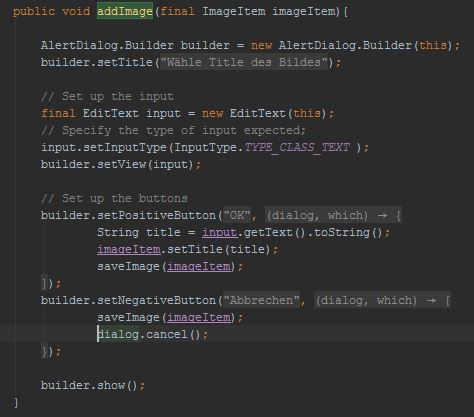
\includegraphics[width=0.65\textwidth]{images/Dialog}
\caption{Bild teilen der Klasse Piccer}
\end{figure}

\begin{lstlisting}
public void addImage(final ImageItem imageItem){

    AlertDialog.Builder builder = new AlertDialog.Builder(this);
    builder.setTitle(R.string.pleaseSelectName);

    // Set up the input
    final EditText input = new EditText(this);
    // Specify the type of input expected;
    input.setInputType(InputType.TYPE_CLASS_TEXT );
    builder.setView(input);

    // Set up the buttons
    builder.setPositiveButton(R.string.ok, new DialogInterface.OnClickListener() {
        @Override
        public void onClick(DialogInterface dialog, int which) {
            String title = input.getText().toString();
            imageItem.setTitle(title);
            saveImage(imageItem);
        }
    });
    builder.setNegativeButton(R.string.abort, new DialogInterface.OnClickListener() {
        @Override
        public void onClick(DialogInterface dialog, int which) {
            saveImage(imageItem);
            dialog.cancel();
        }
    });

    builder.show();
}
\end{lstlisting}
\subsection{Löschen von Bildern}
\subsection{Laden von Thumbnails QUELLTEXT BSP}
Ein großes Problem ist es Bilder in einer Liste anzuzeigen,
da diese erst von der Festplatte geladen werden und eine große Menge von Daten darstellen.
Dadurch kann eine lange Ladezeit entstehen,
wodurch das Scrollen der Liste anfängt zu ruckeln.
Um dieses Problem zu lösen gibt es mehrere Möglichkeiten.
Einerseits kann das Bild redundant abgespeichert werden.
Dabei wird eine deutlich kleinere Kopie des Bildes redundant gespeichert.
Dies verkürzt die Ladezeit des Bildes, löst aber nicht immer das Problem.
Auf einem Smartphone mit einer sehr langsamen Festplatte kann es immer noch zu langen Ladezeiten kommen.
Eine zweite Möglichkeit besteht darin, alle Bilder zu Beginn der Anwendung in den Hauptspeicher zu laden.
Allerdings haben viele Smartphone nur einen begrenzten Arbeitsspeicher, wodurch bei einer 
zu großen Liste die Anwendung abbricht.

Deshalb werden in der \enquote{Piccer} Anwendungen die Thumbnails asynchron auf einem separaten Thread geladen.
Dabei wird auch nicht das komplette Bild geladen sondern nur ein eine komprimierte Version.
Um nicht bereits geladene Bilder erneut laden zu müssen,
hat die Klasse ImageItem ein privates statisches Attribut, welches die bereits geladenen Thumbnails zwischenspeichert.
Dieses Attribut wird als Cache bezeichnet, es kümmert sich darum, dass Bilder die häufiger 
benötigt werden länger gespeichert werden als Bilder die nur einmal geladen werden.
Der Cache hat einen begrenzten Speicherbereich, sobald dieser voll ist, beginnt der Cache
damit Bilder, die nicht oft benötigt werden, zu verwerfen.
Dadurch kann es nicht passieren, dass entweder die Liste ins Stocken gerät oder der Speicher überläuft.

\subsection{Rotieren von Bildern QUELLTEXT}
Um ein Bild zu rotieren, muss es anschließend auch in der Datei gespeichert werden.
Dieser Vorgang dauert recht lange, denn das Bild muss geladen, gedreht und wieder gespeichert werden.
Die meiste Zeit davon wird allerdings zum Laden und speichern benötigt.
Deshalb wird in der Applikation \enquote{Piccer} nur der ImageView eines Bildes gedreht.
Anschließend wird auf einem eigenen Thread das Bild geladen, gedreht und gespeichert.

